\documentclass{article}
\usepackage[margin=2.5cm, top=4cm, headheight=25pt]{geometry}
\usepackage{amsmath, amssymb, enumitem, fancyhdr, graphicx}
\usepackage[indent=20pt]{parskip}
\usepackage[hidelinks]{hyperref}
\usepackage{xcolor}
\usepackage{listings}
\usepackage{subcaption}
\usepackage{url}
\usepackage[most]{tcolorbox}
\usepackage{lastpage}

\tcbuselibrary{listingsutf8} % Support for lstlistings within tcolorbox

\newtcolorbox[auto counter, number within=section]{question}[1][]{%
    colframe=gray!80,                      % Dark gray frame
    colback=gray!5,                       % Light gray background
    coltitle=black,                        % Black title
    title=\textbf{Question~\thetcbcounter}, % Bold title
    fonttitle=\bfseries\large,             % Subtle title font size
    rounded corners,                   % Slightly more rounded corners
    boxrule=0.25mm,                         % Thinner border for a sleek look
    enhanced,                              % Enhanced box features
    attach boxed title to top left={xshift=2mm, yshift=-2mm},
    boxed title style={colframe=gray!80, colback=gray!5, boxrule=0.25mm},
    % Title styling
    #1
}

\bibliographystyle{IEEEtran}
\graphicspath{{./images/}}

% -- Custom Variables --
\def\me{Rajdeep Gill 7934493}
\def\course{ECE 3760}
\def\labsection{A01}
\def\labno{1}
\def\title{Log Book}

% -- Styling for code snippets --
\lstset{
    basicstyle=\ttfamily\small,           % Basic font style
    keywordstyle=\color{blue},            % Keywords color
    commentstyle=\color{gray},            % Comments color
    stringstyle=\color{teal},             % Strings color
    numbers=left,                         % Line numbers on the left
    numberstyle=\tiny\color{gray},        % Line number style
    stepnumber=1,                         % Line number step
    numbersep=10pt,                       % Space between line numbers and code
    backgroundcolor=\color{lightgray!10}, % Background color
    frame=single,                         % Adds a frame around the code
    breaklines=true,                      % Line breaking for long lines
    captionpos=b,                         % Caption position
    showspaces=false,                     % Don't show spaces
    showstringspaces=false                % Don't show spaces in strings
}
\renewcommand{\lstlistingname}{Code Snippet}

\renewcommand{\arraystretch}{1.2} % For less-ugly tables
\setlength\parindent{0pt}

%----- Samples 
% Questions:
%   \begin{question}[title=Custom Question Title]
%       Question details
%   \end{question}

% Tables:
%   \begin{table}[htbp]
%       \centering
%       \caption{Table Caption}
%       \begin{tabular}{ll}
%           \toprule
%           \textbf{Column 1} & \textbf{Column 2} \\
%           \midrule
%           Row 1 & Row 2 \\
%           Row 3 & Row 4 \\
%           \bottomrule
%       \end{tabular}
%   \end{table} 

% Figures:
%   Single figure:
%       \begin{figure}[htbp]
%           \centering
%           \includegraphics[width=0.5\textwidth]{example-image}
%           \caption{Figure Caption}
%       \end{figure}
%   Multiple figures:
%       \begin{figure}[htbp]
%           \centering
%           \begin{subfigure}[b]{0.5\textwidth}
%               \includegraphics[width=\textwidth]{example-image-a}
%               \caption{First subfigure}
%           \end{subfigure}
%           \begin{subfigure}[b]{0.5\textwidth}
%               \includegraphics[width=\textwidth]{example-image-b}
%               \caption{Second subfigure}
%           \end{subfigure}
%           \caption{Main figure}
%       \end{figure}

\newcommand{\logbookentry}[2]{
    \subsection*{#1 \hfill \textit{#2}} 
}

\begin{document}

% --------------------------------------------------------------------------------
% TITLE
% --------------------------------------------------------------------------------

\begin{center}
    \huge \title

    \vspace{2mm}
    \hrule

    \vspace{4mm}
    \large \me

    \vspace{2mm}
    \large \course~\labsection

    \vspace{2mm}
    \today
\end{center}

\vspace{4mm}

% --------------------------------------------------------------------------------
% END TITLE
% --------------------------------------------------------------------------------
\vspace{1cm}
\newpage

\pagestyle{fancy}
\fancyhead[L]{\large Logbook}
\fancyhead[R]{\large \me}

\fancyfoot[C]{Page \thepage~of~\pageref{LastPage}}

% --------------------------------------------------------------------------------
% BODY
% --------------------------------------------------------------------------------
\section{Log Entries}

\logbookentry{Lab 1 Entry}{January 20, 2025}
Recieved the board, soldered pins to the board and ensured that the board was working and no short circuits were present.

Installed platformio on VSCode and ensured the extension was working correctly by running a simple serial print program on the board.

The program was first built and then uploaded to the board, and got a successful message in the console as seen in \autoref{fig:success_upload}.

\begin{figure}[ht!]
    \centering
    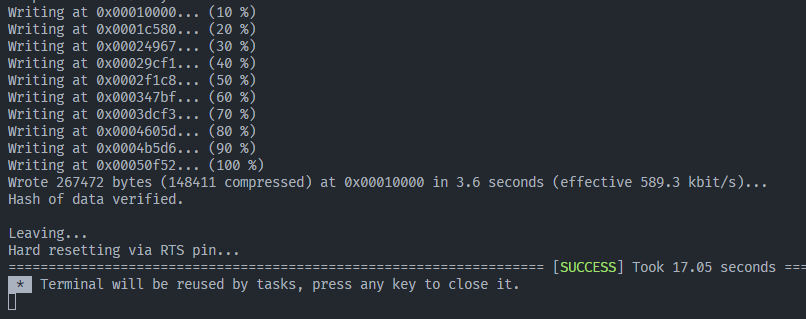
\includegraphics[width=0.75\textwidth]{success_upload.png}
    \caption{Successful upload message in console}
    \label{fig:success_upload}
\end{figure}

\logbookentry{Design Ideas}{January 20, 2025}
During the lab, discussed some ideas for the project. Talked about the basic requirements, what potential ways we can meet the requirements. Need to do more research on how curling actually works to get a better idea of what someone would need to comminicate with their team members to ensure a successful game.

Currently thinking of the skip having a device that can communicate with the two sweepers, having a speed up and slow down button for the sweepers to adjust their speed. The skip would also have a button to indicate when to stop sweeping. On the sweepers side, they would have an LED or a speedometer esque led display to show them how fast they should be sweeping. Since different players might need to sweep at different rates, need to differentiate somehow between the two sweepers. Maybe have two of the same device, but with different colored LEDs or something to indicate which sweeper the skip is talking to. For example, a left and right sweeper device, that connects to the respective sweeper. 

\logbookentry{Individual Design Brainstorming}{January 26, 2025}
A rough sketch of the design I had come up with is provided below. Essentially two sets of controles will be present on the skip's device, one for each sweeper. Along with a display made of LED lights, or other visual indicators to reflect what the sweepers are seeing on there device. 3 buttons will be present, speed up, slow down and an immediate stop button. On the sweeper's device, a line of LED lights or other visual indicators to show a level for the sweeper to sweep at. The skip will be able to adjust the level of the sweeper, and the sweeper will be able to see the level they should be sweeping at.

\begin{figure}[ht!]
    \centering
    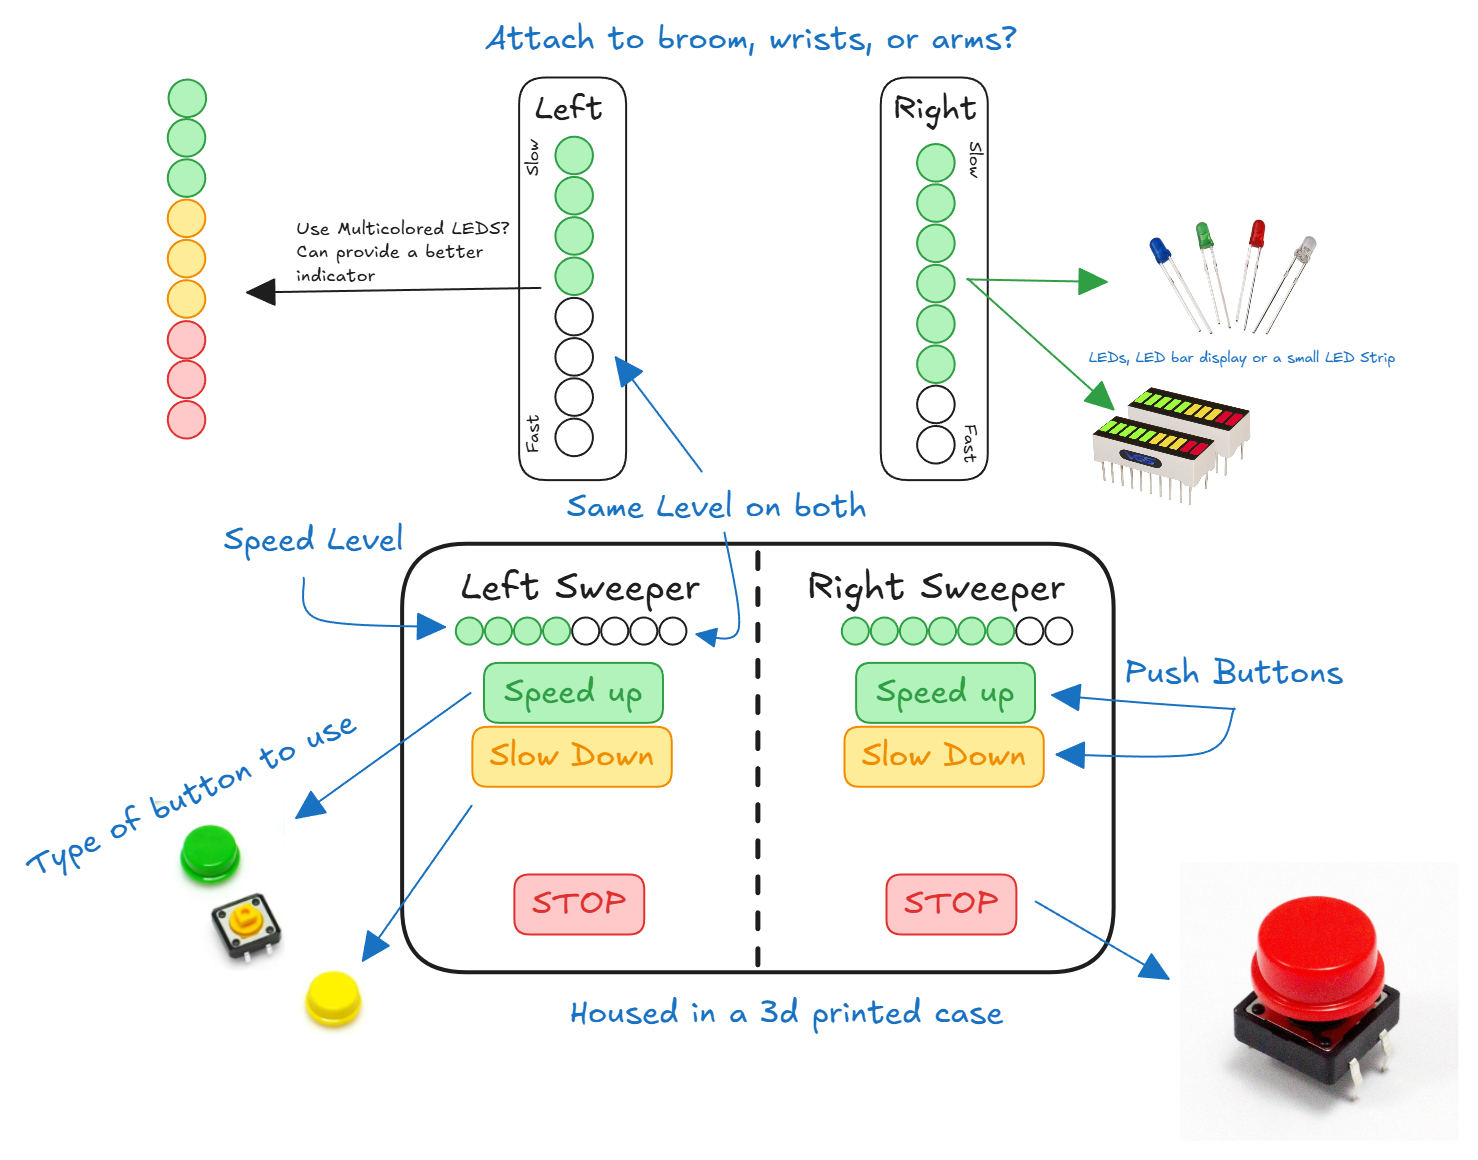
\includegraphics[width=0.6\textwidth]{design_idea1.png}
    \caption{Rough sketch of the design}
\end{figure}
\newpage
The communication between the devices can be done via WiFi as it would have sufficient range to cover the play area. A packet/message structure will need to be defined to ensure the messages are read correctly and by the proper device. A simple message structure could be as follows:

\begin{verbatim}
    <sweeper_id, message_data>
\end{verbatim}
Where \texttt{sweeper\_id} can be a 1 bit for which sweeper, if more than 2 sweepers are present, then we could use 2, 3, 4 bits to represent the sweeper. The message data for each message can be as simple as the level of speed to set the sweeper to, and the sweeper would reply back with an ACK message of the current level they are at to ensure proper synchronization. A simple message-communication diagram is shown below.

\begin{figure}[ht!]
    \centering
    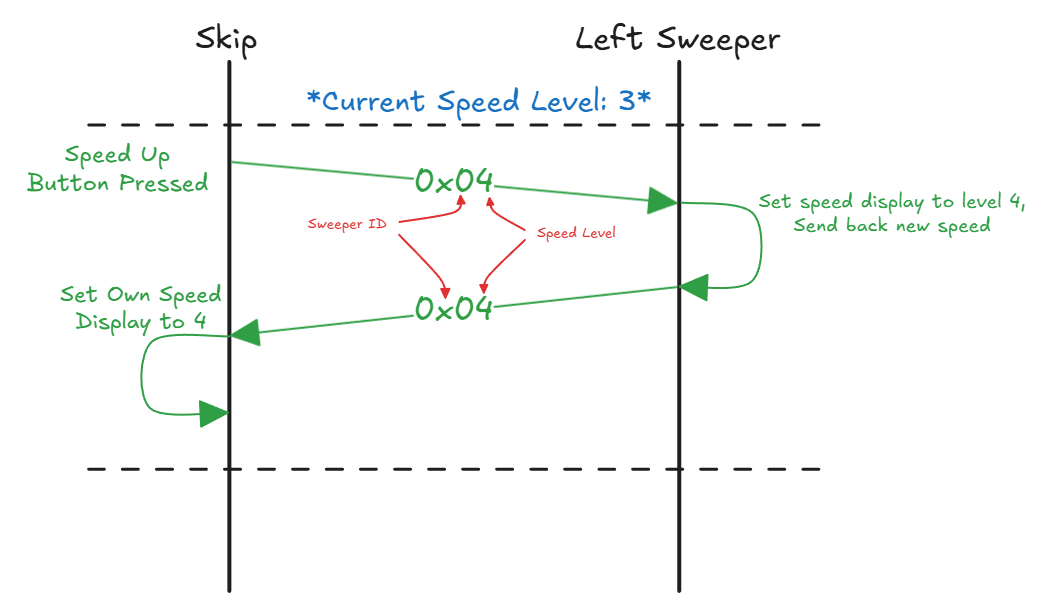
\includegraphics[width=0.6\textwidth]{message_structure_idea.png}
    \caption{Message communication diagram}
\end{figure}

Both sweepers will actively listen to all messages and only act when the \texttt{sweeper\_id} matches their own. This will ensure that the skip can communicate with both sweepers at the same time.

\logbookentry{A Compact Design}{January 28, 2025}
A more compact device for the skip could be used, where a switch can be used to toggle between the two sweepers. This would reduce the size of the device, and essentially reduces the number of components to just half. On the sweepers device a small vibration motor can be used to indicate a message has just arrived. A rough sketch is shown below for the more compact design.
\begin{figure}[ht!]
    \centering
    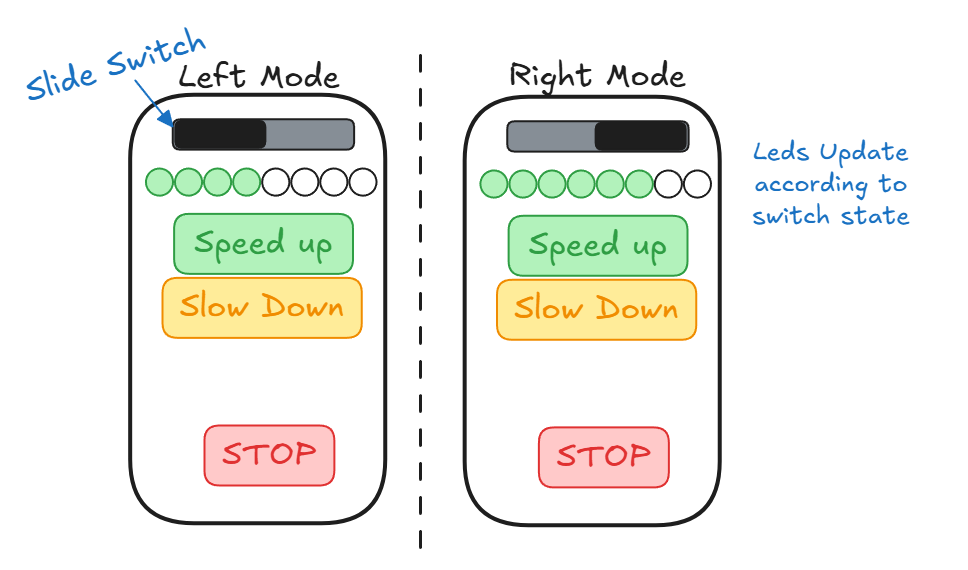
\includegraphics[width=0.6\textwidth]{design_idea2.png}
    \caption{More compact design idea}
\end{figure}

The downside I can see with this is that the skip would need to swap between the two sweepers, which could be a bit cumbersome at times. However, the size reduction could be worth it, and reduced cost of the device. It also will have less LEDs so power consumption could be reduced as well.



% --------------------------------------------------------------------------------
% END BODY
% --------------------------------------------------------------------------------

\end{document}
